\documentclass[]{article}
\usepackage{lmodern}
\usepackage{amssymb,amsmath}
\usepackage{ifxetex,ifluatex}
\usepackage{fixltx2e} % provides \textsubscript
\ifnum 0\ifxetex 1\fi\ifluatex 1\fi=0 % if pdftex
  \usepackage[T1]{fontenc}
  \usepackage[utf8]{inputenc}
\else % if luatex or xelatex
  \ifxetex
    \usepackage{mathspec}
  \else
    \usepackage{fontspec}
  \fi
  \defaultfontfeatures{Ligatures=TeX,Scale=MatchLowercase}
\fi
% use upquote if available, for straight quotes in verbatim environments
\IfFileExists{upquote.sty}{\usepackage{upquote}}{}
% use microtype if available
\IfFileExists{microtype.sty}{%
\usepackage{microtype}
\UseMicrotypeSet[protrusion]{basicmath} % disable protrusion for tt fonts
}{}
\usepackage[margin=1in]{geometry}
\usepackage{hyperref}
\hypersetup{unicode=true,
            pdfborder={0 0 0},
            breaklinks=true}
\urlstyle{same}  % don't use monospace font for urls
\usepackage{graphicx,grffile}
\makeatletter
\def\maxwidth{\ifdim\Gin@nat@width>\linewidth\linewidth\else\Gin@nat@width\fi}
\def\maxheight{\ifdim\Gin@nat@height>\textheight\textheight\else\Gin@nat@height\fi}
\makeatother
% Scale images if necessary, so that they will not overflow the page
% margins by default, and it is still possible to overwrite the defaults
% using explicit options in \includegraphics[width, height, ...]{}
\setkeys{Gin}{width=\maxwidth,height=\maxheight,keepaspectratio}
\IfFileExists{parskip.sty}{%
\usepackage{parskip}
}{% else
\setlength{\parindent}{0pt}
\setlength{\parskip}{6pt plus 2pt minus 1pt}
}
\setlength{\emergencystretch}{3em}  % prevent overfull lines
\providecommand{\tightlist}{%
  \setlength{\itemsep}{0pt}\setlength{\parskip}{0pt}}
\setcounter{secnumdepth}{0}
% Redefines (sub)paragraphs to behave more like sections
\ifx\paragraph\undefined\else
\let\oldparagraph\paragraph
\renewcommand{\paragraph}[1]{\oldparagraph{#1}\mbox{}}
\fi
\ifx\subparagraph\undefined\else
\let\oldsubparagraph\subparagraph
\renewcommand{\subparagraph}[1]{\oldsubparagraph{#1}\mbox{}}
\fi

%%% Use protect on footnotes to avoid problems with footnotes in titles
\let\rmarkdownfootnote\footnote%
\def\footnote{\protect\rmarkdownfootnote}

%%% Change title format to be more compact
\usepackage{titling}

% Create subtitle command for use in maketitle
\newcommand{\subtitle}[1]{
  \posttitle{
    \begin{center}\large#1\end{center}
    }
}

\setlength{\droptitle}{-2em}

  \title{}
    \pretitle{\vspace{\droptitle}}
  \posttitle{}
    \author{}
    \preauthor{}\postauthor{}
    \date{}
    \predate{}\postdate{}
  

\begin{document}

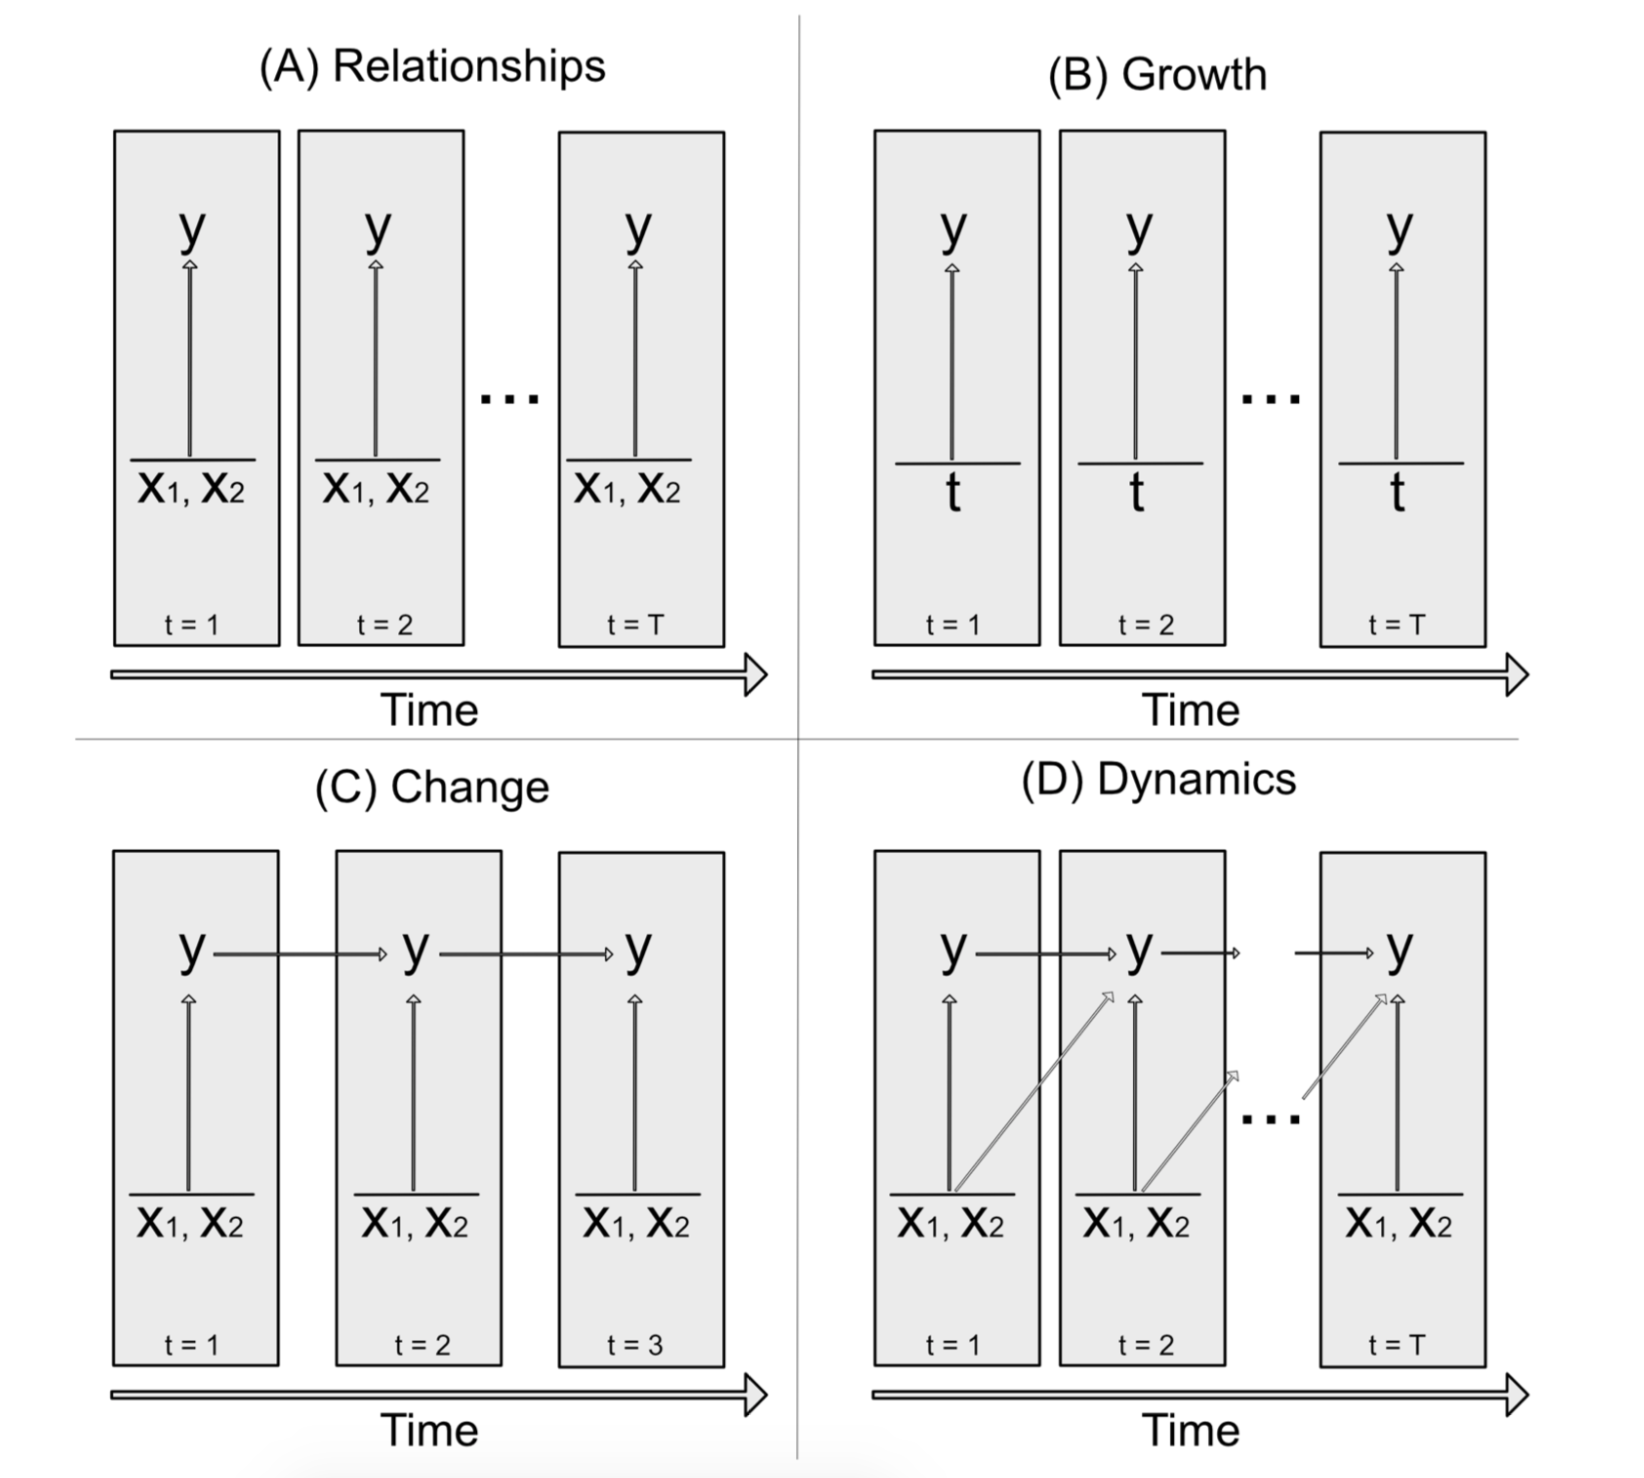
\includegraphics{https://github.com/Cdishop/longitudinal_cookbook/raw/master/misc/common_models.png}

Please see questions at bottom after reading.

\hypertarget{paper-sections}{%
\section{Paper Sections}\label{paper-sections}}

\begin{itemize}
\tightlist
\item
  Hook
\item
  Introduction

  \begin{itemize}
  \tightlist
  \item
    Quick bit about the hype of longitudinal and process
  \item
    Introduce inferences
  \end{itemize}
\item
  Inference sections with examples
\item
  End

  \begin{itemize}
  \tightlist
  \item
    These were abstracted to form common research questions. There are
    other aspects that we did not cover because they have not received
    attention.

    \begin{itemize}
    \tightlist
    \item
      Tiny discussion of these as a teaser
    \end{itemize}
  \end{itemize}
\end{itemize}

\hypertarget{hook}{%
\section{Hook}\label{hook}}

We -- organizational researchers -- are increasingly interested in
process inferences. Emergence, growth, change, dynamics, and
explanations over time are becoming explicit in organizational theory.
Empirical tests of our theories now commonly collect longitudinal data
sets with a growing number of time points. New statistical techniques to
support inferences with these longitudinal data structures emerge every
year. Computational modelers have made their role for refining process
knowledge clear and their frequency appears to be growing. Across these
developments, however, researchers present seemingly unrelated
hypotheses and employ diverse statistical approaches -- which impedes
any unity about how to demonstrate and support a process inference.

Researchers that study process are therefore in a similar state to those
that were interested in multilevel phenomena two decades ago. Then, we
debated how to measure multilevel constructs, justify aggregation, and
analyze multilevel models (Klein \& Kozlowski, 2000), and our research
advanced only after developing consensus. Now, we conceptualize and
model different aspects of process -- such as change, growth, or
dynamics -- without a shared understanding of the diverse approaches and
pitfalls of each. We need to clearly understand how researchers'
approach and justify the variety of inferences they make about the
processes in longitudinal data -- and the drawbacks of each -- to avoid
inferential errors and to develop the process knowledge so many authors
call for (zillion cites).

Our goal is to explain these various approaches and provide a guide for
researchers who want to study process. Researchers tend to focus on an
inference, or set of inferences, related to one dimension at play in
longitudinal data (e.g., growth), and this results in seemingly
unrelated hypotheses and model applications across research streams. We
unpack the core inference underlying each, discuss their differences,
provide examples and direct readers to possible statistical models, and
show how they can be used to cumulatively understand process.

\hypertarget{intro}{%
\section{Intro}\label{intro}}

Hype process. Introduce inferences.

\hypertarget{relationships}{%
\section{Relationships}\label{relationships}}

\hypertarget{inference-1}{%
\subsection{Inference 1}\label{inference-1}}

The relationship of one or more predictor variables with a response
variable over time.

\hypertarget{examples}{%
\subsubsection{Examples}\label{examples}}

\hypertarget{hypotheses}{%
\paragraph{Hypotheses}\label{hypotheses}}

@barnes2011 and @chi2015 present hypotheses that are consistent with a
relationships inference. @barnes2011 predict a negative relationship
between poor sleep and cognitive self control. Similarly, @chi2015
hypothesize that daily negative mood negatively relates to daily task
performance.

\hypertarget{longitudinal-data-structure}{%
\paragraph{Longitudinal Data
Structure}\label{longitudinal-data-structure}}

Researchers that infer relationships over time either a) measure their
variables at the same time points or b) treat the data as if they were
measured as so by the constraints of their analysis. @barnes2011 give an
example of the former; they measure sleep and cognitive self control
every morning for five consecutive days (study 4). @chi2015, as an
example of the latter, measure negative mood in the morning and task
performance in the afternoon -- but these variables are treated as if
they were taken at the same time (e.g., day 4) when entered into their
analysis (described later).

There is no limit to the number of possible time points, but studies of
this type typically collect between three and ten repeated measurements.
Our examples above measure their variables once per day, but other
frequencies could also be used. Methods literature typically recommends
that researchers maintain the same interval between each measurement
across their study, but this can be difficult when studies last longer
than a week. For example, @chi2015 take their measurements for ten work
days. In the middle of those assessments, however, their sample
employees go home for the weekend and are not measured. The space,
therefore, between \(t\) and \(t + 1\) is not the same across their
analysis. Finally, our organizational literature almost always takes
measures on more than one unit across time.

\hypertarget{models}{%
\paragraph{Models}\label{models}}

Both @barnes2011 and @chi2015 use hiearchical linear modeling (HLM) --
also known as multi-level or random coefficient models -- to estimate
the parameters that generate their observed data. Random coefficient
models assume that their random effects are distributed
\(N(\gamma, \sigma^2)\) -- but this statement is easier to understand
with a contrast. Imagine that everyone in the sample receives their own
\(X_t\) on \(Y_t\) effect and we then summarize those effects by taking
their average. HLM, conversely, estimates one \(X_t\) on \(Y_t\) effect
across units (people) but does so by imposing a normality constraint.
Finally, @barnes2011 and @chi2015 use models that fall into the broader
time-varying analysis class because their measurements of \(X\) are
allowed to vary over time. In time-invariant analyses, conversely,
values of the covariate remain stable (e.g., gender).

\hypertarget{pitfalls-and-recommendations}{%
\subsubsection{Pitfalls and
Recommendations}\label{pitfalls-and-recommendations}}

What can go wrong. Recommendation. Why.

\hypertarget{growth}{%
\section{Growth}\label{growth}}

\hypertarget{inference-1-1}{%
\subsection{Inference 1}\label{inference-1-1}}

What is the level of a construct at a given point in time?

\hypertarget{examples-1}{%
\subsubsection{Examples}\label{examples-1}}

\hypertarget{hypotheses-1}{%
\paragraph{Hypotheses}\label{hypotheses-1}}

There are few (if any) studies that make direct predictions about
construct levels at certain time points. Almost every longitudinal
study, however, estimates an intercept term to approximate the answer.
These terms are then discussed in the context of broader growth
inferences that we discuss below.

\hypertarget{longitudinal-data-structure-1}{%
\paragraph{Longitudinal Data
Structure}\label{longitudinal-data-structure-1}}

This inference requires several repeated measures on one variable. For
example, @zhu2016 measure work adjustment once a month for nine months
(among expatriates) and @jones2016 measure concealing behaviors (among
pregnant women) every week -- but it is not clear for how long they do
so.

\hypertarget{models-1}{%
\paragraph{Models}\label{models-1}}

@zhu2016 use HLM to estimate their parmaters, whereas @jones2016 do so
in a structural equation modeling framework. As stated, researchers are
interested in an intercept estimate for this inference, and although
they can place it on any time point, researchers typically use their
first observation. In SEM, the intercept is a latent variable regressed
on either an observed indicator (again, usually the first observation)
or its latent equivalent. @jones2016, for example, regress their latent
concealing behaviors intercept term on the latent variable for
concealing behaviors at time one. In HLM, the investigator first creates
a variable that represents time and then regresses the outcome on this
time indicator to estimate an intercept term. For example, @zhu2016
regress work adjustment on time using HLM to estimate its initial level.

\hypertarget{pitfalls-and-recommendations-1}{%
\subsubsection{Pitfalls and
Recommendations}\label{pitfalls-and-recommendations-1}}

What can go wrong. Recommendations. Why.

\hypertarget{inference-2}{%
\subsection{Inference 2}\label{inference-2}}

What are the patterns of a trajectory or trajectories across time? How
does the construct change over time?

\hypertarget{examples-2}{%
\subsubsection{Examples}\label{examples-2}}

\hypertarget{hypotheses-2}{%
\paragraph{Hypotheses}\label{hypotheses-2}}

@zhu2016 predict that expatriate work adjustment follows a positive
trajectory, increasing over the time of the assignment. Similarly,
@jones2016 hypothesize that concealing behaviors will have negative
slopes over time.

\hypertarget{longitudinal-data-structure-2}{%
\paragraph{Longitudinal Data
Structure}\label{longitudinal-data-structure-2}}

As with our previous inference, the only requirement here is a repeated
assessment on one variable over several time points -- both @zhu2016 and
@jones2016 meet these requirements.

\hypertarget{models-2}{%
\paragraph{Models}\label{models-2}}

Researchers use slope terms in their models for making inferences about
trajectory patterns. In HLM, the same procedure we described above --
regressing the outcome on time -- also provides a slope estimate.
Typically researchers do not allow their slope estimates to vary over
units, but the models can easily support random slope terms. @zhu2016,
for example, estimate a random slope effect by regressing work
adjustment on time. In SEM, a latent slope term is regressed onto all
time points except for the time point that was used by the latent
intercept term. @jones2016 regress a latent concealing behaviors slope
term on latent concealing behaviors at all time points beyond \(t_1\).

Researchers may also be interested in curvilinear slopes. The only
additional requirement for doing so is to create other time indicators
with respect to the higher order polynomial. @zhu2016, for example,
included linear, quadratic, and cubic time variables to estimate
different slope curves. Note that these are still ``linear'' processes
because they are linear in parameters.

\hypertarget{pitfalls-and-recommendations-2}{%
\subsubsection{Pitfalls and
Recommendations}\label{pitfalls-and-recommendations-2}}

What can go wrong. Recommendations. Why.

\hypertarget{inference-3}{%
\subsection{Inference 3}\label{inference-3}}

Are there between person differences in trajectories or levels?

\hypertarget{examples-3}{%
\subsubsection{Examples}\label{examples-3}}

\hypertarget{hypotheses-3}{%
\paragraph{Hypotheses}\label{hypotheses-3}}

Similar to our first growth inference, researchers rarely make a direct
prediction about between person differences in trajectory or level, but
it is almost always included as part of a larger growth analysis.

\hypertarget{longitudinal-data-structure-3}{%
\paragraph{Longitudinal Data
Structure}\label{longitudinal-data-structure-3}}

We now require repeated observations on multiple units to examine
between person (unit) differences. For example, @zhu2016 collect data
from 179 expatriates across nine consecutive months.

\hypertarget{models-3}{%
\paragraph{Models}\label{models-3}}

Models that estimate intercept or slope terms also estimate a variance
on those terms, and these are then subjected to significance tests. When
the variance on the intercept is significant, that is taken to mean that
there are between unit differences in intercept (levels), whereas
significant variance estimates on the slope terms indicates between unit
differences in slope (trajectory). @zhu2016 use HLM to estimate the
variance on their intercept and slope terms and find evidence of between
person differences in work adjustment intercept (level) and slope
(trajectory).

\hypertarget{pitfalls-and-recommendations-3}{%
\subsubsection{Pitfalls and
Recommendations}\label{pitfalls-and-recommendations-3}}

What can go wrong. Recommendations. Why.

\hypertarget{inference-4}{%
\subsection{Inference 4}\label{inference-4}}

How is the level of a construct related to the trajectory of the same or
different constructs? What is the correlation between intercept and
slope terms?

\hypertarget{examples-4}{%
\subsubsection{Examples}\label{examples-4}}

\hypertarget{hypotheses-4}{%
\paragraph{Hypotheses}\label{hypotheses-4}}

@schaubroeck2016 predict that initial levels of peer leader's
transformational leadership will positively relate to the slope of
employee beliefs. @zhu2016 hypothesize that initial level of expatriate
work adjustment is negatively related to the speed of change in work
adjustment. Notice that the first prediction is about how the level of
one construct is related to the slope of another, whereas the second
focuses only on a single variable. Although it is uncommon in our
literature, developmental researchers will also predict associations
between slope and the final -- rather than initial -- observation.

\hypertarget{longitudinal-data-structure-4}{%
\paragraph{Longitudinal Data
Structure}\label{longitudinal-data-structure-4}}

Data structures that researchers use to examine this inference are
consistent with what we have already reviewed. @schaubroeck2016 measured
transformational leadership and employee beliefs at three time points.
Their time two assessment was 10 weeks after their first observation,
whereas their final measurement was taken 10 months after their second
observation. That is, the data structure for their respective time
points were \(t\), \(t + 10\), and \(t + 40\). As stated above, @zhu2016
collected data once a month for nine months.

\hypertarget{models-4}{%
\paragraph{Models}\label{models-4}}

Both HLM and SEM provide estimates of the covariance between the
intercept and slope terms discussed above, and this covariance indicates
the association between level and trajectory. For example, @zhu2016
report a negative covariance estimate betwen the initial level of
expatriate work adjustment (intercept) and its linear trajectory over
time (slope). As stated, researchers can also examine this association
but among the level of one variable and the trajectory of a different
variable. @schaubroeck2016 report an estimate of the relationship
between transformational leadership intercept and employee beliefs
slope. It is often helpful to generate predicted values using the
analysis estimates and then plot the levels and trajectories to
interpret them appropriately.

\hypertarget{pitfalls-and-recommendations-4}{%
\subsubsection{Pitfalls and
Recommendations}\label{pitfalls-and-recommendations-4}}

What can go wrong. Recommendations. Why.

\hypertarget{inference-5}{%
\subsection{Inference 5}\label{inference-5}}

What inter-individual characteristics relate to intra-individual
differences in level or slope?

\hypertarget{examples-5}{%
\subsubsection{Examples}\label{examples-5}}

\hypertarget{hypotheses-5}{%
\paragraph{Hypotheses}\label{hypotheses-5}}

Inferences of this type take the form of stable unit effects and their
relationship with trajectory or level. @li2017 predict a positive
relationship between job strain and job complexity trajectory. @zhu2016
hypothesize that the trajectory of expatriate work adjustment is
positively related to perceived career instrumentality. Finally,
@jones2016 make two inferences of this type: contextual support is a)
negatively related to average levels of concealing but b) positively
related to the slope of concealing.

\hypertarget{longitudinal-data-structures}{%
\paragraph{Longitudinal Data
Structures}\label{longitudinal-data-structures}}

We discussed the data structures for @zhu2016 and @jones2016 above.
@li2017 use a similar design but their data are collected once per year.
Job complexity is measured once every year for three years, and job
strain is measured once at the final time point (year 3).

\hypertarget{models-5}{%
\paragraph{Models}\label{models-5}}

Both @li2017 and @zhu2016 use HLM to estimate their parameters, whereas
@jones2016 do so with SEM. In these models, the intercept or slope terms
discussed above are regressed onto the inter-individual characteristic.
For example, @li2017 report the estimate of job strain predicting job
complexity trajectory and @zhu2016 do the same but for career
instrumentality and job complexity trajectory. In the SEM framework,
@jones2016 report estimates of contextual support predicting concealing
slope and intercept. Note that these models fit into the broader
time-invariant analysis class that contrast with the time-variant
covariates analyses discussed earlier.

\hypertarget{pitfalls-and-recommendations-5}{%
\subsubsection{Pitfalls and
Recommendations}\label{pitfalls-and-recommendations-5}}

What can go wrong. Recommendations. Why.

\hypertarget{change}{%
\section{Change}\label{change}}

\hypertarget{inference-1-2}{%
\subsection{Inference 1}\label{inference-1-2}}

How are the changes of one variable associated with changes in another
over time?

\hypertarget{examples-6}{%
\subsubsection{Examples}\label{examples-6}}

\hypertarget{hypotheses-6}{%
\paragraph{Hypotheses}\label{hypotheses-6}}

Change inferences are similar to relationship inferences in that they
relate a predictor to a response at the same time point, but the
researcher now wants to know whether the predictor is associated with an
increase or decrease of the outcome. For example, @johnson2014 predict
that, within individuals, exhibiting daily procedural justice behavior
is associated with an increase in resource depletion. Similarly,
@Lanaj2016 hypothesize that, within individuals, transformational
leadership is associated with a decrease in negative affect.

\hypertarget{longitudinal-data-structures-1}{%
\paragraph{Longitudinal Data
Structures}\label{longitudinal-data-structures-1}}

@johnson2014 measured justice behavior and resource depletion in the
afternoon of 10 consecutive workdays. @Lanaj2016 measured their
variables at different frequencies. They measured transformational
leadership and negative affect in the afternoon of 15 consecutive
workdays, but they also took an additional measurement of negative
affect every morning -- creating a data structure of three variables:
negative affect from \(t\) to \(t + 15\), transformational leadership
from \(t\) to \(t + 15\) and morning negative affect from \(t\) to
\(t + 15\). That is, they essentially doubled the time points of
negative affect -- from \(t\) to \(t + 30\) by measuring it twice as
frequently.

\hypertarget{models-6}{%
\paragraph{Models}\label{models-6}}

@johnson2014 and @Lanaj2016 employ HLM change models that are consistent
with our literature's preference for using partialed values of the
outcome variable rather than difference scores. In models of this type,
researchers regress their outcome on the predictor at the same time
point and the prior value of the outcome variable. For example,
@johnson2014 regressed resource depletion at time \(t\) on 1) procedural
justice behavior at time \(t\) and 2) resource depletion at time
\(t-1\); they then report the relationship between justice behavior and
resource depletion change. Similarly, @Lanaj2016 regress negative affect
at time \(t\) on 1) transformational leadership at time \(t\) and 2)
negative affect at time \(t-1\) (i.e., morning negative affect) and
report the association between transformational leadership and affect
change. Note that, due to the different data sampling strategies,
@johnson2014 reports change from the prior day, whereas @Lanaj2016
report change from the morning to afternoon.

\hypertarget{pitfalls-and-recommendations-6}{%
\subsubsection{Pitfalls and
Recommendations}\label{pitfalls-and-recommendations-6}}

What can go wrong. Recommendations. Why.

\hypertarget{dynamics}{%
\section{Dynamics}\label{dynamics}}

The core concept is: how are prior states related to future states?

\hypertarget{inference-1-3}{%
\subsection{Inference 1}\label{inference-1-3}}

How is one variable related to its future self?

\hypertarget{examples-7}{%
\subsubsection{Examples}\label{examples-7}}

\hypertarget{hypotheses-7}{%
\paragraph{Hypotheses}\label{hypotheses-7}}

\hypertarget{longitudinal-data-structures-2}{%
\paragraph{Longitudinal Data
Structures}\label{longitudinal-data-structures-2}}

\hypertarget{models-7}{%
\paragraph{Models}\label{models-7}}

\hypertarget{pitfalls-and-recommendations-7}{%
\subsubsection{Pitfalls and
Recommendations}\label{pitfalls-and-recommendations-7}}

\hypertarget{inference-2-1}{%
\subsection{Inference 2}\label{inference-2-1}}

How is one variable related to a different variable in the future?

\hypertarget{examples-8}{%
\subsubsection{Examples}\label{examples-8}}

\hypertarget{hypotheses-8}{%
\paragraph{Hypotheses}\label{hypotheses-8}}

@gabriel2014 hypothesize that perceived P-O fit is positively related to
subsequent positive affect.

\hypertarget{longitudinal-data-structure-5}{%
\paragraph{Longitudinal Data
Structure}\label{longitudinal-data-structure-5}}

@gabriel2014 measured perceived P-O fit and positive affect five times
per day for 10 consecutive work days.

\hypertarget{models-8}{%
\paragraph{Models}\label{models-8}}

Researchers that use models related to this inference regress their
outcome at time \(t\) on a prior value of the independent variable.
@gabriel2014 do so using HLM and regress perceive P-O fit at time \(t\)
on 1) positive affect at time \(t-1\) and 2) perceived P-O fit at time
\(t-1\).

\hypertarget{pitfalls-and-recommendations-8}{%
\subsubsection{Pitfalls and
Recommendations}\label{pitfalls-and-recommendations-8}}

What can go wrong. Recommendations. Why.

\hypertarget{inference-3-1}{%
\subsection{Inference 3}\label{inference-3-1}}

Directionality -- what is the relationship direction among a set of
variables?

\hypertarget{examples-9}{%
\subsubsection{Examples}\label{examples-9}}

\hypertarget{hypotheses-9}{%
\paragraph{Hypotheses}\label{hypotheses-9}}

A directionality inference is typically explored using a pair of dynamic
hypotheses. For example, @hardy2018 predict that 1) prior self efficacy
negatively relates to subsequent meta cognition and 2) prior meta
cognition positively relates to subsequent self efficacy. Similarly,
@matthews2014 contrast two theories, one that predicts that work-family
conflict is negatively related to subsequent well-being, whereas the
other predicts that well-being is negatively related to work-family
conflict.

\hypertarget{longitudinal-data-structures-3}{%
\paragraph{Longitudinal Data
Structures}\label{longitudinal-data-structures-3}}

@hardy2018 measured self efficacy and meta cognition after five evenly
spaced computer game trails -- although they also measured baseline self
efficacy. @matthews2014 assessed work-family conflict and well-being
concurrently at three points in time: \(t\), \(t+1\), and \(t+7\) where
the intervals are months -- meaning that the final survey was assessed
six months after the survey before it.

\hypertarget{models-9}{%
\paragraph{Models}\label{models-9}}

Both @hardy2018 and @matthews2014 use an SEM approach to estimate their
parameters, but @matthews2014 restrict their model to a path analysis.
Their modeling strategies are the same as those just presented, but they
examine them as a set to explore the relationship direction among their
variables. @matthews2014 find significant effects in both directions --
WFC predicting subsequent well-being and well-being predicting
subsequent WFC -- and therefore suggest that the relationship works in
both directions. @hardy2018 also report the estimates of self efficacy
predicting subsequent meta cognition and vice versa, but only find
significant effects for the latter. They conclude that ``self-regulatory
processes (i.e., exploration and meta cognition) positively influenced
subsequent self-efficacy\ldots{}In contrast, we only found limited
support for the notion that self-efficacy significantly influences
subsequent self-regulated learning processes'' (p.~24).

\hypertarget{pitfalls-and-recommendations-9}{%
\subsubsection{Pitfalls and
Recommendations}\label{pitfalls-and-recommendations-9}}

What can go wrong. Recommendations. Why.

\hypertarget{inference-4-1}{%
\subsection{Inference 4}\label{inference-4-1}}

Reciprocal -- Is the pattern of relationships reciprocal, such that one
variable influences another, and this latter variable then goes back to
influence the first?

\hypertarget{examples-10}{%
\subsubsection{Examples}\label{examples-10}}

\hypertarget{hypotheses-10}{%
\paragraph{Hypotheses}\label{hypotheses-10}}

@kaltiainen2017 present a set of hypotheses to explore reciprocal
dynamics among justice perceptions and trust. They predict that
``process justice perceptions and cognitive trust have positive
reciprocal relations over time. Specifically, planning stage (time 1)
process justice (cognitive trust) perceptions will have a positive
relationship with subsequent post-merger (time 2) cognitive trust
(process justice) perceptions, which in turn will have a positive
relationship with later post-merger (time 3) process justice (cognitive
trust) perceptions'' (p.~idk).

\hypertarget{longitudinal-data-structure-6}{%
\paragraph{Longitudinal Data
Structure}\label{longitudinal-data-structure-6}}

They assess cognitive trust and justice perceptions once a year for
three years.

\hypertarget{models-10}{%
\paragraph{Models}\label{models-10}}

@kaltiainen2017 evaluate a number of models but find best fit for a
model that includes reciprocal relationships among justice and trust. In
that model, trust at time \(t\) is regressed on trust at time \(t-1\)
and justice at time \(t-1\), and justice at time \(t\) is regressed on
trust at time \(t-1\) and justice at time \(t-1\). They find significant
cross-lag effects for trust on justice at all times but only one
significant cross-lag effect of justice on trust, and ultimately
conclude that ``the justice \({\Rightarrow}\) trust \({\Rightarrow}\)
justice reciprocal relationship was supported but the trust
\({\Rightarrow}\) justice \({\Rightarrow}\) trust relationship was not
supported as the relationship between justice at time 2 and cognitive
trust at time 3 was not statistically significant'' (p.~14).

\hypertarget{pitfalls-and-recommendations-10}{%
\subsubsection{Pitfalls and
Recommendations}\label{pitfalls-and-recommendations-10}}

What can go wrong. Recommendations. Why.

\hypertarget{inference-5-1}{%
\subsection{Inference 5}\label{inference-5-1}}

Mediation -- one variable influences an outcome through an intermediate
variable

\hypertarget{things-to-notice-and-questions}{%
\section{Things to notice and
questions}\label{things-to-notice-and-questions}}

\begin{enumerate}
\def\labelenumi{\arabic{enumi})}
\item
  Not going example by example, I am combining them.

  \begin{itemize}
  \tightlist
  \item
    Originally I thought it would be more clear this way, but I could be
    wrong. I do not have enough examples to pair every inference with
    its own unique empirical example.
  \end{itemize}
\item
  Pitfalls and recommendations after each inference (as I did
  here\ldots{}) or after each entire inference section (i.e., one for
  relationships, one for growth, etc.)?
\item
  ``We'' or ``they'' phrasing?

  \begin{itemize}
  \item
    I.e., ``we as a field typically do this\ldots{}'' or ``researchers
    tend to do this\ldots{}''
  \item
    Not for stylistic reasons but for authoritative reasons.
  \end{itemize}
\item
  Several issues that came up while writing the data structures sections

  \begin{itemize}
  \item
    \begin{enumerate}
    \def\labelenumii{\arabic{enumii})}
    \tightlist
    \item
      They are repetitive
    \end{enumerate}
  \item
    \begin{enumerate}
    \def\labelenumii{\arabic{enumii})}
    \setcounter{enumii}{1}
    \tightlist
    \item
      Each example has their own issue (e.g., spacing between t and t +
      1 isn't consistent, or the variables were measured at different
      frequencies). If I bring them up out of the blue it is really easy
      to lose the reader.
    \end{enumerate}
  \item
    Solutions

    \begin{itemize}
    \item
      I could write one data structure piece per inference section
      rather than one per inference
    \item
      I could skip data structures in the inference examples -- just
      provide hypotheses and models -- and then give them their own
      section later
    \item
      I could give pictures like figure 1 in Xu and DeShon in each
      inference example section and then give data structures and issues
      their own section later. That is, in the examples I simply speak
      about hypotheses and models as if every study measured their
      variables from \(t\) to \(t + 10\) on the same interval. Then, at
      the end I come back with data collection problems/discrepancies I
      noticed in the articles. I like this option.
    \end{itemize}
  \end{itemize}
\end{enumerate}


\end{document}
